\sectionCenteredToc{Введение}

В современном мире backend-разработки микросервисная архитектура уверенно позиционируется как <<де-факто>> стандарт для проектирования масштабных проектов. Основополагающим принципом данной архитектуры является декомпозиция логики приложения на автономные сервисы, взаимодействующие друг с другом посредством сетевых запросов. Преимуществами такого подхода выступают гибкость масштабирования, повышенная надежность и отказоустойчивость, структурированность кода.
Однако, наряду с перечисленными достоинствами, микросервисная архитектура влечет за собой и ряд сопутствующих сложностей. К ним относятся накладные расходы на сетевое взаимодействие, сериализацию и десериализацию данных.

Одним из популярных решений для сериализации данных в микросервисной архитектуре является Protocol Buffers, разработанный компанией Google. Этот протокол представляет собой высокопроизводительный инструмент для сериализации структурированных данных, обеспечивая компактное и быстрое представление информации. Protocol Buffers использует двоичный формат, что позволяет минимизировать затраты ресурсов при передаче данных.

Несмотря на преимущества Protocol Buffers, при работе с большими объемами данных возникает проблема производительности десериализации вложенных полей. Десериализация вложенных полей подразумевает рекурсивный процесс извлечения и обработки вложенных структур данных. В случае больших объемов вложенных данных этот процесс может стать ресурсоемким, негативно влияя на общую производительность системы.

Предлагаемое в данной работе решение "ленивой" десериализации вложенных полей Protocol Buffers позволит оптимизировать производительность обработки данных в микросервисной архитектуре, повысив ее эффективность при работе с большими объемами информации.

В рамках данной дипломной работы производится определение и описание задач, в которых возможно применение предложенной оптимизации ленивой десериализации вложенных полей Protocol Buffers, разработка программного модуля, осуществляющего ленивую десериализацию вложенных полей Protocol Buffers, проведение замеров производительности предложенного решения на различных тестовых задачах, а также сравнение производительности ленивой десериализации с традиционным подходом десериализации всех вложенных полей.

Результаты исследования могут быть применены для разработки высокопроизводительных микросервисных систем, способных эффективно обрабатывать большие объемы данных.

Работа выполнена самостоятельно, проведён анализ оригинальности в системе <<Антиплагиат>>. Цитирования обозначены ссылками на публикации, указанные в <<Списке использованной литературы>>.

\begin{figure}[ht]
    \centering
    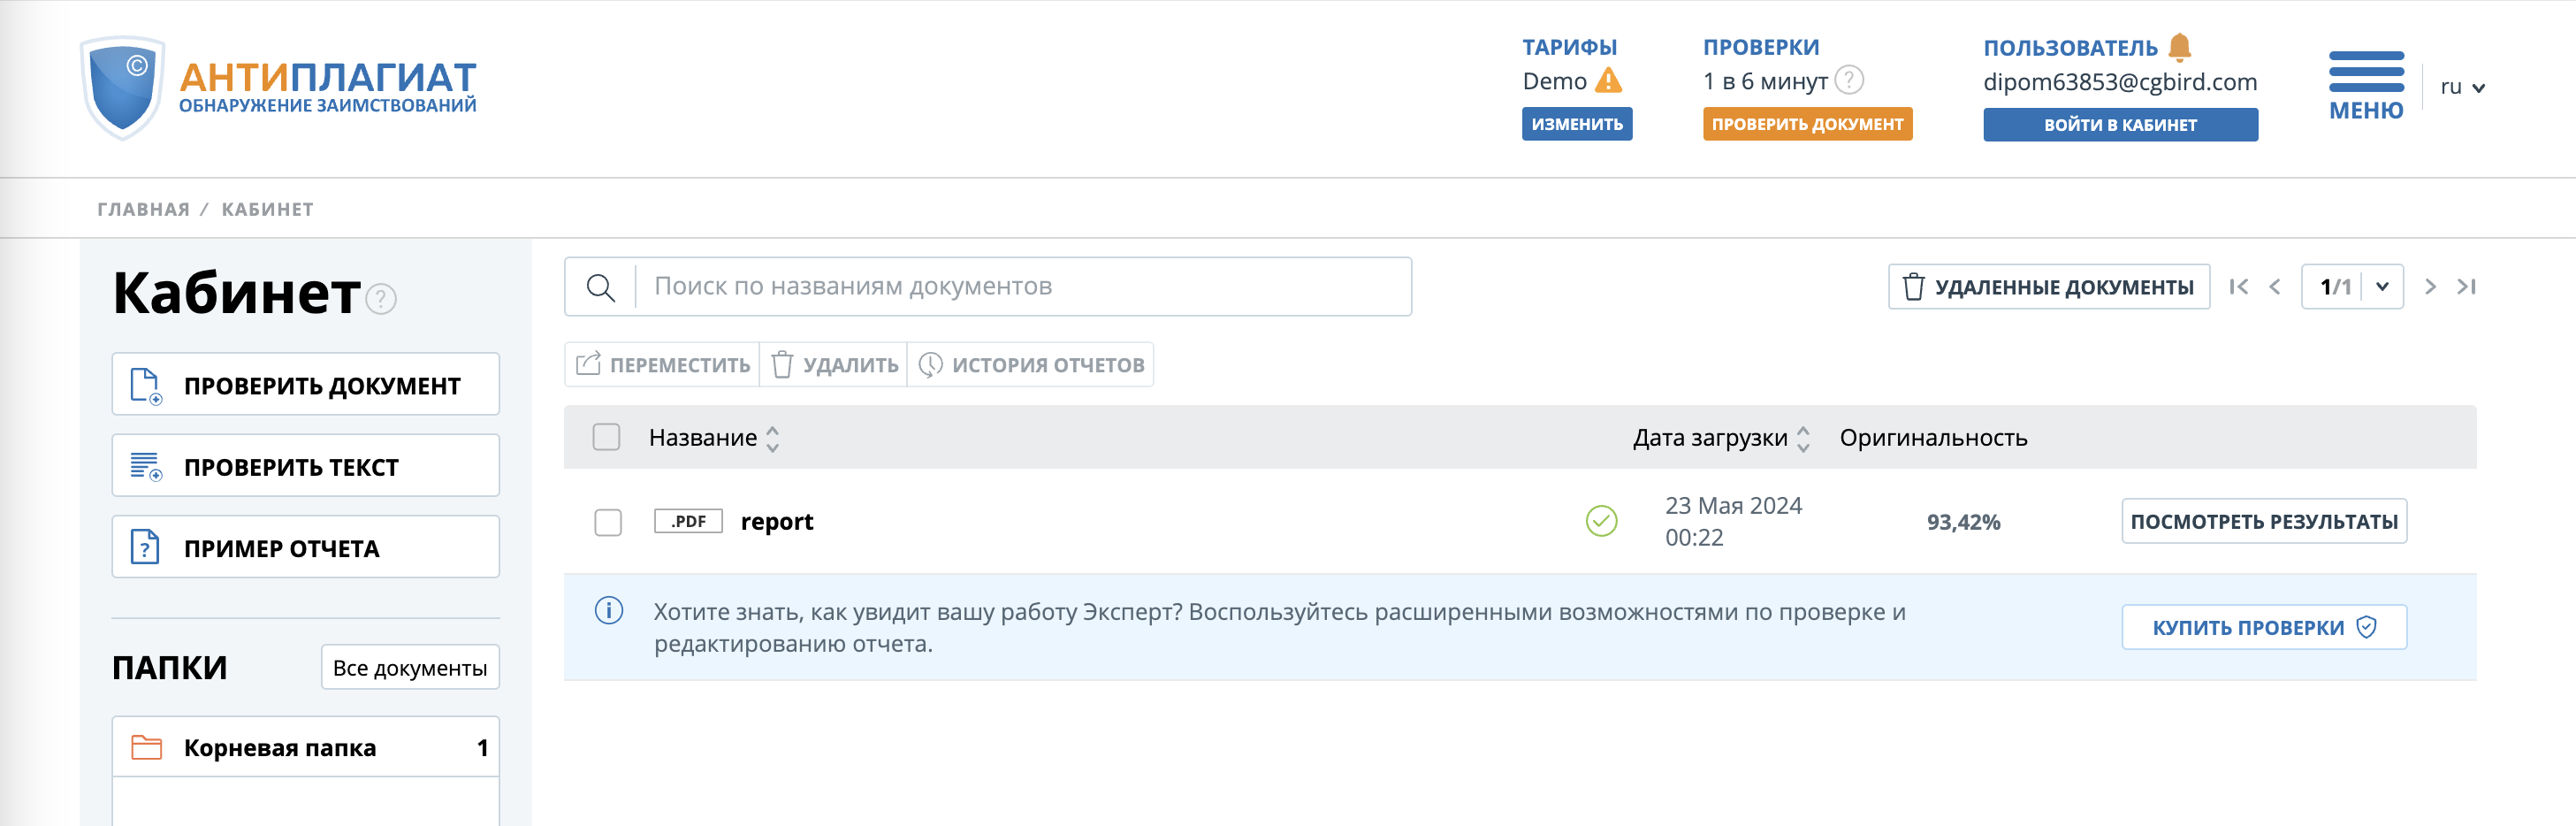
\includegraphics[width=0.85\linewidth]{\commonSecPathPrefix/sec_intro_attachments/antiplagiat.png}
\end{figure}
